\documentclass[a4paper, 11pt]{article}
\usepackage{etex}
%packages indispensables 
\usepackage[utf8]{inputenc}
\usepackage{lmodern}
\usepackage{graphicx}
%packages utiles
\usepackage{alltt} %program code
\usepackage{enumerate}
\usepackage{amssymb} %lettres mathématiques
\usepackage{amsmath}
\usepackage{amsthm}
\usepackage{bussproofs} %derivation
\usepackage{hyperref} %to write path.
\usepackage{color} % colouring text
\usepackage{tabularx} % table
\usepackage{fancyvrb}
{\renewcommand{\arraystretch}{1.5}
\usepackage[toc,page]{appendix}
\usepackage{cite}


%%%%%%%%%%%%%%%%%%%%%%%%%%%%%%%%%%%%
\usepackage{tikz} % to draw diagrams
\usetikzlibrary{arrows,shapes}
\usetikzlibrary{trees,positioning,fit}
\tikzstyle{decision} = [diamond, draw, fill=blue!20, 
    text width=4.5em, text badly centered, node distance=3cm, inner sep=0pt]
\tikzstyle{block} = [rectangle, draw, fill=blue!20, 
    text width=5em, text centered, rounded corners, minimum height=4em]
\tikzstyle{line}=[draw]
\tikzstyle{cloud} = [draw, ellipse,fill=red!20, node distance=3cm,
    minimum height=2em]
%%%%%%%%%%%%%%%%%%%%%%%%%%%%%%%%%%%%    
\usepackage{pgfplots}
%margin definition
%\usepackage{geometry} 
%\geometry{hmargin=2cm,vmargin=2cm} 

% commands for presentation
\theoremstyle{plain}
\newtheorem*{thm}{Theorem}
\newtheorem*{corollary}{Corollary}
\newtheorem*{prop}{Proposition}
\newtheorem*{stat}{Statement}
\theoremstyle{definition}
\newtheorem*{mydef}{Definition}
\newtheorem*{property}{Property}
\theoremstyle{remark}
\newtheorem*{remark}{Remark}
\newtheorem*{example}{Example}

% commands
\newcommand\sep{\mbox{ } | \mbox{ }}

%title,author,date
\title{HOL4-Beagle, an implementation of a higher-order to first-order translation}
\author{Thibault Gauthier}
\date{\today}

\begin{document}
\newcommand{\slice}[4]{
  \pgfmathparse{0.5*#1+0.5*#2}
  \let\midangle\pgfmathresult
  % slice
  \draw[thick,fill=black!10] (0,0) -- (#1:1) arc (#1:#2:1) -- cycle;
  % outer label
  \node[label=\midangle:#4] at (\midangle:1) {};
  % inner label
  \pgfmathparse{min((#2-#1-10)/110*(-0.3),0)}
  \let\temp\pgfmathresult
  \pgfmathparse{max(\temp,-0.5) + 0.8}
  \let\innerpos\pgfmathresult
  \node at (\midangle:\innerpos) {#3};
}
\maketitle 


\begin{abstract}
\par The interactive theorem prover HOL4 is interfaced with an external automated theorem prover Beagle. The necessary work involves the implementation of a sound translation from the polymorphic higher-order logic of HOL4 to the monomorphic first-order logic of Beagle.
\par  Performance of the HOL4-Beagle system is evaluated against problems solved by the internal prover METIS$\_$TAC during HOL4 build. It is shown that Beagle proves 80$\%$ of 271 translated theorems in 15 seconds of real time on one CPU.
\end{abstract}
.
\pagebreak
\tableofcontents
\pagebreak

\section{Introduction}
\subsection{Context}
Interactive theorem provers are used by researchers for certifying proofs of problems such as the Kepler conjecture and modelling complex algorithms or systems. The main weakness of these tools is that they need a lot of human guidance. To solve this problem, internal automated methods were created but they are usually limited to specific problems. Therefore, it is a natural thing to enhance them with automated theorem provers which tackle a wide range of first-order problems automatically.

\subsection{Interactive provers and automated provers comparison} 
We present here the strength and the weakness of both these tools.

\noindent \begin{tabularx}{\textwidth}{ |c|X|X| }
  \hline
  & Interactive theorem provers & Automated theorem provers\\
  \hline  
  Provers & HOL4, HOL/Isabelle, HOL light, Coq, \ldots 
  & Beagle, SPASS, Vampire, E-prover, E-Darwin, \ldots                                           \\
  \hline  
  Input & Mathematical problems directly match their higher-order logic format.
  & Mathematical problems need to be translated to their first-order logic format.
  \\  
  \hline
  Efficiency & Need human guidance. Have internal automated procedures but are very specialized. & Automatically prove a wide range of first-order problems.\\
  \hline
  Reliability & Are based on easily verifiable small kernel. & Proving their relatively long code is a bit harder and has to be repeated for each new version. Another approach is to check their proof output "a posteriori".\\
  \hline
\end{tabularx}
\begin{remark}
It is worth to mention that there exists other kind of automated theorem provers such as SMT solvers.
\end{remark}
\subsection{General problem}
\subsubsection{Problem statement}
\textit{Problem:}
\\ HOL4 is an interactive theorem prover. It has an internal first-order prover METIS$\_$TAC. But this internal prover does not deal with arithmetic without user-provided theorems.

\noindent \textit{Solution:}
\\A new tactic called BEAGLE$\_$TAC is created. 
It calls an external prover Beagle that was designed to cope with arithmetic problems. 
\\
\subsubsection{The HOL4-Beagle interaction diagram}
  This is how BEAGLE{\_}TAC globally works.
  
\begin{tikzpicture}[node distance = 2cm, auto]
  % Place nodes
  \node [cloud] (conjecture) {conjecture};
  \node [block, right of=conjecture,  node distance=3cm] (HOL1) 
  {first-order translation};
  \node [block, right of=HOL1, node distance=3cm] (TFF1) 
  {problem file};
  \node [block, right of=TFF1, node distance=3cm] (Beagle) 
  {automatic proof search};
  \node [block, below of=TFF1, node distance=2cm] (TFF2) 
  {proof file};  
  \node [block, below of=HOL1, node distance=2cm] (HOL2) 
  {proof replaying};
  \node [cloud, below of=conjecture, node distance=2cm] (theorem) 
  {theorem};
  \node [label=HOL4, draw=black, ultra thick, 
  fit=(conjecture) (theorem) (HOL1) (HOL2)] {}; 
  \node [label=TFF format interface, draw=black, ultra thick, fit=(TFF1) (TFF2)] 
  {}; 
  \node [label=Beagle, draw=black, ultra thick, fit=(Beagle)] {}; 
  % Draw edges
  \draw [-to,black,ultra thick] (conjecture) -- (HOL1);
  \draw [-to,black,ultra thick] (HOL1) -- (TFF1);
  \draw [-to,,black,ultra thick] (TFF1) -- (Beagle);
  \draw [-to,black,ultra thick,dashed] (Beagle) -- (TFF2);
  \draw [-to,black,ultra thick,dashed] (TFF2) -- (HOL2);
  \draw [-to,black,ultra thick,dashed] (HOL2) -- (theorem);
  \draw [-to,black,ultra thick] (Beagle.south) to       [out=270,in=270] (theorem.south);
\end{tikzpicture}

\begin{remark} The plain arrows are currently implemented, so BEAGLE{\_}TAC can only be used as an oracle.
The first-order translation was proved, thus the conjecture is true if Beagle returns the conjecture as a theorem and if you believe that the printing part (second arrow) and Beagle are sound.
\end{remark} 

\begin{remark}
The TFF format will be used as an interface between HOL4 and Beagle. This has some advantages:
\begin{enumerate}
\item The problem file created by HOL4 can be given to any other automated theorem prover that can read TFF problems.
\item The proof file created by Beagle (work in progress) could be tested within any other TFF proof checker.
\end{enumerate}
\end{remark} 

\subsection{Structure of this report}
Up to Section 4, we present the different tools we used in our project. The Section 5 (Translation) explains the main part of our project. Then, we put the problem into perspective in Section 6,7,8.


\section{The TFF(TPTP) format}
The TPTP website (Thousands Problems for Theorem Provers) (\path{http://www.cs.miami.edu/~tptp/}) provides a database for theorem provers to be tested against. A TPTP format is human-readable and non specific prover dependent. 
\\The syntax of a problem can be checked online there: \\\path{http://www.cs.miami.edu/~tptp/cgi-bin/SystemB4TPTP}. 
\\Some automated theorem provers can be called on any problem there: \\\path{http://www.cs.miami.edu/~tptp/cgi-bin/SystemOnTPTP}.

\subsection{TFF format}
The TFF format is one of the format used to write these problems, it represents first-order, typed and arithmetic formulas. 
\begin{mydef} (TFF type)
\\A TFF type is inductively defined by :
\[type,ty_1,\ldots,ty_n,\ldots := d \sep u \sep (ty_1 * \ldots * ty_m) > type\]
where $d$ is a defined type and $u$ a user-defined type.
\end{mydef}



\section{The HOL4 interactive theorem prover}
\subsection{General ideas}
HOL4 is an interactive theorem prover that deals with higher-order logic, which is close to the language mathematicians use to express their formulas. It is based on the functional programming and type checking language SML. To learn more about programming in HOL4, you can read the Kananaskis documentation.
 
\subsection{HOL4 type and formula representation}
   
\begin{mydef} (HOL4 types)
\\The set of all types is inductively defined by:
 \[type,ty_1,\ldots,ty_n,\ldots := b \sep p \sep (op,[ty_1,\ldots,ty_m])\] 
where $b$ is a basic type, $p$ is a polymorphic type and $op$  is a type operator.
\end{mydef}
 
\begin{remark} 
$(fun,[a,b])$ is the HOL4 internal representation of $a \rightarrow b$.
\end{remark}

\begin{remark} 
To say that a variable $f$ has type $t$, we write $f:t$.
\end{remark}

\begin{mydef} (HOL4 Formula)
\\This definition is based on the typed $\lambda$-calculus:
\[ f,g := c \sep v \sep n \sep (g)\ f \sep \lambda v. f\]
where  $c$ is a constant, $v$ is a variable and $n$ a positive integer.
\\There are type constraints when building $(g)\ f$.
\end{mydef}

\begin{remark}
A variable has a name and a type that can be accessed by respectively calling $name\_of$ and $type\_of$.
\end{remark}

\begin{example}
$\forall x,\mbox{ } x = 0$ is represented in HOL4 by $(!)\ \lambda x. ((=)\ x)\ 0$ .
\end{example}

\subsection{Useful SML types}
  Here is a list of SML types created in HOL4 and their intended use:
\begin {enumerate}  
  \item Term ($term$)
\\This is the type of HOL4 formulas described above. 
  \item Goal ($goal = (term\mbox{ }list * term)$)
\\Used for conjectures in a sequent form.
  \item Theorem ($thm$) 
\\Theorems are represented in a sequent form. A theorem may be created by any function that returns a theorem.
  \item Rule ($rule = thm \rightarrow thm$)
\\Using a rule is the most common way to create theorems. Rules can be used to simulate steps in a derivation. 
  \item Conversion ($conv = term \rightarrow thm$)
\\Takes a term and returns a theorem of the form A |- term = term. Conversions will be used to rewrite terms inside a theorem.
  \item Tactic ($tactic = goal \rightarrow goal\mbox{ }list * (thm\mbox{ }list \rightarrow thm)$)
\\Takes a goal and returns a goal list and a way to reconstruct the proof when every goal in the goal list happens to be proved. Its used in interactive mode, so that the user can construct the proof backwards.
  \item Problem ($thm\mbox{ }list * goal$)
\\This is not a type by itself but it will represent the problem we want to solve.
\end{enumerate}

\begin{remark} Except for the $thm$ type, there is no control whether you use a type in the intended way or not.
\end{remark}

\subsection{Soundness}
  Since $thm$ is an SML abstract type, only reserved functions can return the $thm$ type. The number of these functions is small and all these functions are simple enough, so they can be checked by a human. Then, new variables of type $thm$ can only be created by one of these functions. That is why every new variable of type $thm$ is a theorem.

\subsection{One easy proof}
Here is an example of a derivation and how it can be simulated in HOL4 using forward and backward reasoning.

\begin{prooftree}
\AxiomC{$A \vdash A$}
\AxiomC{$B \vdash B$}
\RightLabel{$\wedge_i$}
\BinaryInfC{$A,B \vdash A \wedge B$}
\RightLabel{$\Rightarrow_i$}
\UnaryInfC{$A \vdash B \Rightarrow (A \wedge B) $}
\RightLabel{$\Rightarrow_i$}
\UnaryInfC{$\vdash A \Rightarrow (B \Rightarrow (A \wedge B)) $}
\end{prooftree}

\scriptsize
\begin{Verbatim}[frame=single]
(* forward proof *)
val th1 = ASSUME ``A:bool``;
val th2 = ASSUME ``B:bool``;
val th3 = CONJ th1 th2;
val th4 = DISCH ``B:bool`` th3;
val th5 = DISCH ``A:bool`` th4;
\end{Verbatim} 
\begin{Verbatim}[frame=single]
(* backward proof (using the interactive goal stack) *)
g(`A ==> B ==> A /\ B `);
e(DISCH_TAC);
e(DISCH_TAC);
e(CONJ_TAC);
e(ACCEPT_TAC th1);is
e(ACCEPT_TAC th2);
\end{Verbatim} 
\normalsize

\subsection{Derivation format}
You can use the TFF format to encode derivations. For more information, look at \path{http://www.cs.miami.edu/~tptp/TPTP/QuickGuide/Derivations.html.}is

\section{The Beagle automated theorem prover}
Beagle is an automated theorem prover that deals with typed first-order arithmetic formulas. It translates the problem into a clause set (e.g. $\lbrace x \vee g(x), f(y) \vee \neg x \rbrace$).
\\It returns that the clause set is either unsatisfiable, satisfiable or unknown.

\begin{remark}
To look deeper in the Beagle calculus, which contains rules such as superposition, you can read ~\cite{Waldmann13}.
\end{remark}

\subsection{Derivation search in Beagle}
\subsubsection{Saturation loop (no Split)} 
Beagle uses two clause sets, the new clause set (NCS) and the old clause set (OCS). The OCS is initially empty. The NCS is initially the one created by the normalisation step.
\\Let us consider that the Split rule is not used ,the main loop can be represented by this diagram:
  
\begin{tikzpicture}[auto]
  % Place nodes
  \node [cloud] (NCS) {new clause set};
  \node [cloud, above of=NCS, node distance = 2cm] (init) {TFF file};
  \node [label = below:2, cloud, below of=NCS, node distance = 3cm] (OCS) {old clause set};
  % Draw edges
  \draw[-to,black,ultra thick] (NCS.east) to [out=0,in=0] node[name=down]{1} (OCS.east) ;
  \draw[-to,black,ultra thick] (OCS.west) to [out=180,in=180] node[name=up]{3} (NCS.west)  ;
  \draw[-to,black,ultra thick] (init) -- node[name=what]{parsing and normalisation} (NCS)  ;  
  % Place boxes
  \node [block, right of=down, node distance=2cm] (rightbox)  
  {Move a clause};  
  \node [block, below of=OCS, node distance=2cm] (downbox)  
  {Apply any possible rules};      
  \node [block, left of=up, node distance=2cm] (leftbox)  
  {Move all created clauses};   
\end{tikzpicture}
  
These are the steps of the saturation loop:  
\begin{enumerate}  
\item  Move a clause from the new clause set into the old clause set (using a good ordering)
\item  Derive all consequences from the application of any rule (except for the Split rule) to any subset of the old clause set. You only have to check the subsets that contain the moving clause.
\item Move all created consequences into the new clause set.
\end{enumerate}

\begin{stat}
After each saturation loop, the old clause set is closed under 
the reunion of the old clause set and the new clause set.
\end{stat} 

\subsubsection{A special rule: Split}

\begin{mydef} (saturation loop state)
Let us represent a saturation loop state by a triplet (c, OCS ,NCS) where c is the clause which was moved from NCS to OCS. 
\end{mydef} 
 
\begin{mydef} (Split)
A Split is defined by this inference step. 
\\Let $a_1 \vee a_2 \vee \ldots a_N$ a clause.

\begin{prooftree}
\AxiomC{$(a_1 \vee a_2 \vee \ldots a_N,OCS,NCS)$}
\RightLabel{$Split$}
\UnaryInfC{$(a_1,OCS,NCS),(a_2,OCS,NCS),\ldots,(a_N,OCS,NCS)$}  
\end{prooftree}  
   
\end{mydef}

\begin{remark} This is the only rule which creates new saturation loops from one saturation loop, other rules only modify the saturation they are in.
\end{remark}
\begin{remark} The proof can be represented by a tree, each node being a saturation loop.
\end{remark}
  
\subsubsection{Termination}

There are mostly three possibilities that can happen in that point.
\begin{enumerate}
\item If every leaf OCS contains a contradiction then the clause set is \textbf{unsatisfiable}. (Beagle rule set is refutation-complete)
\item If there exists a saturated clause set which does not contains any contradiction:
\subitem If the initial clause set was sufficiently complete, then the status of this problem is \textbf{satisfiable}.
\subitem If the initial clause set was not sufficiently complete, then the status of this problem is \textbf{unknown}.
\item The computation may go on forever. (The first-order logic is undecidable)
\end{enumerate} 


\section{HOL4 problem translation}

\subsection{Code location}
The code for this translation is located at \path{https://github.com/barakeel/HOLtoTFF}. Some examples can be found in paperexample.sml.

\subsection{Notation}
A term of type bool is called a formula and often written $f$.
\\We write u[t] when a term t is free in a term u. 

\subsection{Atoms for a higher-order formula}
A higher-order formulas can be represented in a way that looks like a first-order formula. From then, atoms can be defined for a higher-order formula.

\begin{mydef} (Atom)
Let $L$ be the set of logical operators. ($\Rightarrow$,$\wedge$,$\ldots$)
\\A term $t$ in a formula $f$ is said to be an atom if it satisfies all these conditions:
\begin{enumerate}
\item [-] Its operator is not a logical operator.
\item [-] For each term that includes this term, his operator is a logical operator. 
\end{enumerate}
\end{mydef}

\subsection{Translation order}
The translation order was thought carefully. It happens in this order: 
\begin{enumerate}    
  \item Monomorphisation. (may be done at anytime but it happens first to improve efficiency \cite{MengP08}.)
  \item Goal negation. 
  \\The goal is rewritten to ([hypotheses, conclusion negation],false).
  Then a conjunction of the new goal and the theorem list returns a single term. 
  \item CNF conversion.
  \item $\lambda$-lifting conversion then CNF conversion. 
  \item Boolean arguments conversion then CNF conversion.
  \\This step is necessary because the TFF format does not accept boolean variables as arguments.
  \item Numeral variables conversion then CNF conversion.  
  \item Clause set tactic. 
  \\ Transform the term into a clause set.      
  \item Higher-order conversion.
  \\ This conversion occurs almost at the end of the translation, it allows us to limit the number of problems that are considered higher-order.(e.g. $\exists f.\ \forall x.\ f\ x = 0$ is not a higher-order formula.)
  \item Numeral functions axioms.
  \\ It has to be done after the higher-order conversion because the $App$ operator produced by the higher-order conversion may be a numeral function. 
  \item Boolean bound variables conversion.  
  \\This step is necessary because the TFF format does not accept quantified boolean variables.
    \item Printing.
    \subitem Variables or constants.  
    \subitem Types.
    \subitem True and false constants.
    \subitem Non-linear integer arithmetic.
\end{enumerate}  
  
\subsection{Monomorphisation}
In this step, provided theorems containing polymorphic types are instantiated in a "clever" way.
  
\begin{example} if we are given a theorem $!x:a.\ C\ x\ x$ and a goal $C \ 42\ 42$ , it is "clever" to instantiate the theorem with the substitution $[a \mapsto num]$. One way of doing this is to find a substitution that matches the type of $C : a \rightarrow a \rightarrow bool$ to the type of $C : num \rightarrow num \rightarrow bool$ and apply this substitution to the theorem.
\end{example}
 
\begin{remark}
If the goal contains polymorphic types, they should be treated as new fresh types with non-polymorphic value.
\end{remark} 
  


\subsubsection{Dependency graph}
In this section, we will present a theoretical representation of our monomorphisation implementation.
\vspace{2mm}

\noindent For every problem, a dependency graph can be defined. 
\begin{mydef} (Dependency graph)
\begin{enumerate}
  \item [-] Nodes are constants in the theorem list or in the goal. Two same constants are represented by different nodes if they are in different theorems or one is in the goal and the other is not.
  \item [-] {\color{blue}Substitution} directed links connect two different constants that verify this properties: 
    \subitem The initial one does not belong to the goal.
    \subitem They have the same name.
    \subitem The type of the destination is a type instance of the type of the origin. 
  \item [-] {\color{green}Binding} undirected links connect two constants that verify this properties: 
    \subitem They are from the same theorem.
    \subitem They share a common polymorphic type.    
\end{enumerate}    
Each substitution links infers a substitution. When there is no ambiguity, we will identify the link and the substitution.
\end{mydef}


\begin{remark}
When drawing a dependency graph or its supergraph, we will draw  constants from the same theorem (or goal) in the same row.
\end{remark}

\noindent \textit{Example of a dependency graph.} 
\begin{center}  
\begin{tikzpicture}[node distance = 3cm, auto]
  \node [cloud, fill=white,node distance = 3cm] (c11) {C: a};
  \node [cloud, fill=white, right of=c11,node distance = 3cm] (c12) {D: a};
  \node [cloud, fill=white, below of=c11,node distance = 1.5cm] (c21) {C: b};
  \node [cloud, fill=white, below of=c12,node distance = 3cm] (c32) {D: num};
  \draw[-to,blue,ultra thick](c11) -- (c21);
  \draw [-to,blue,ultra thick] (c21) -- (c11);
  \draw [-to,blue,ultra thick] (c12) -- (c32);
  \draw [green,ultra thick] (c11) -- (c12);
\end{tikzpicture}
\end{center}

\begin{mydef} (A substitution transformation)
The substitution transformation $\mathcal{T}_s$ of a dependency graph $G$ for a substitution link $\sigma$ from $c$ to $c'$, is defined by:
\[\mathcal{T}_s(G) = G \cup \sigma(c) \]
where the created image stays in the same theorem.
\end{mydef}

\noindent \textit{New dependency graph using the right substitution link as a substitution transformation.}

\begin{center}
\begin{tikzpicture}[node distance = 3cm, auto]
  \node [cloud, fill=white,node distance = 3cm] (c11) {C: a};
  \node [cloud, fill=white, right of=c11,node distance = 3cm] (c12) {D: a};
  \node [cloud, fill=white, right of=c12,node distance = 3cm] (c13) {D: num};
  \node [cloud, fill=white, below of=c11,node distance = 1.5cm] (c21) {C: b};
  \node [cloud, fill=white, below of=c12,node distance = 3cm] (c32) {D: num};
  \draw[-to,blue,ultra thick](c11) -- (c21);
  \draw [-to,blue,ultra thick] (c21) -- (c11);
  \draw [-to,blue,ultra thick] (c12) -- (c32);
  \draw [-to,blue,ultra thick] (c13) -- (c32);
  \draw [green,ultra thick] (c11) -- (c12);
\end{tikzpicture}
\end{center}

\begin{mydef} (A binding transformation)
The binding transformation $\mathcal{T}_b$ of a graph $G$, for a binding link from $c$ to $c'$ and a substitution link $\sigma$ from $c'$ to $c''$, is defined by:
\[\mathcal{T}_b(G) = G \cup \sigma(c) \]
where the created image stays in the same theorem.
\end{mydef}
\noindent \textit{New dependency graph using the binding link and the right substitution link as a binding transformation.}

\begin{center}
\begin{tikzpicture}[node distance = 3cm, auto]
  \node [cloud, fill=white,node distance = 3cm] (c11) {C: a};
  \node [cloud, fill=white, right of=c11,node distance = 3cm] (c12) {D: a};
  \node [cloud, fill=white, right of=c12,node distance = 3cm] (c13) {C: num};
  \node [cloud, fill=white, below of=c11,node distance = 1.5cm] (c21) {C: b};
  \node [cloud, fill=white, below of=c12,node distance = 3cm] (c32) {D: num};
  \draw[-to,blue,ultra thick](c11) -- (c21);
  \draw [-to,blue,ultra thick] (c21) -- (c11);
  \draw [-to,blue,ultra thick] (c12) -- (c32);
  \draw [green,ultra thick] (c11) -- (c12);
\end{tikzpicture}
\end{center}

\begin{mydef} (A graph transformation)
The graph transformation $\mathcal{T}$ is defined by applying all possible substitution transformations and binding transformations simultaneously to a graph $G$. 
\end{mydef}

\noindent \textit{New supergraph using the graph transformation}
\begin{center}  
\begin{tikzpicture}[node distance = 3cm, auto]
  \node [cloud, fill=white,node distance = 3cm] (c11) 
  {C: a,{\color{blue} b},{\color{green} num}};
  \node [cloud, fill=white, right of=c11,node distance = 4cm] (c12) {D: a,{\color{green} b},{\color{blue} num}};
  \node [cloud, fill=white, below of=c11,node distance = 1.5cm] (c21) {C: b,{\color{blue} a}};
  \node [cloud, fill=white, below of=c12,node distance = 3cm] (c32) {D: num};
  \draw[-to,blue,ultra thick](c11) -- (c21);
  \draw [-to,blue,ultra thick] (c21) -- (c11);
  \draw [-to,blue,ultra thick] (c12) -- (c32);
  \draw [green,ultra thick] (c11) -- (c12);
\end{tikzpicture}
\end{center}

\begin{mydef} (Supergraph of a dependency graph)
Let $G$ be a dependency and $G_i$ the dependency graph created after $i$ transformation $\mathcal{T}$. The supergraph $SG_i$ of $G_i$ is defined by:
\begin{enumerate}
  \item [-] Nodes are sets composed of a node in the initial graph $G$ (head node) and all its derived nodes in $G_i$ (tail nodes). They will be called a supernodes.
  \item [-] {\color{blue}Substitution} undirected links connect two nodes $sn_1$ and $sn_2$ when there is at least one  {\color{blue}substitution} link, between a constant in $sn_1$ and a constant in $sn_2$, in $G_i$.
  \item [-] {\color{green}Binding} undirected links connect two nodes $sn_1$ and $sn_2$ when there is at least one {\color{green}binding} link , between a constant in $sn_1$ and a constant in $sn_2$, in $G_i$.
\end{enumerate}    
\end{mydef}

\begin{mydef} (Redundancy)
\\A substitution link is redundant if it has the same origin and induce the same substitution as a substitution link inside the supernode of its origin. From this point, we will not draw redundant substitution link.
\end{mydef}
\noindent \textit{Supergraph at step 1 with a redundant substitution link.}
\\A substitution link inside the super node is exceptionally represented.

\begin{center}
\begin{tikzpicture}[node distance = 3cm, auto]
  % Place nodes
  \node [cloud, fill=white,node distance = 3cm] (c11) 
  {A: a, {\color{red}num}};
  \node [cloud, fill=white, below of=c11,node distance = 1.2cm] (c12) {A: num};
  \draw[-to,blue,ultra thick](c11) to [in=0,out=0] (c12);
  \draw[-to,blue,ultra thick](c11) to [in=40,out=130] (c11);
\end{tikzpicture}
\end{center}

\begin{mydef} (Directable)
\\A graph $G$ is directable if every binding link $b$ can be oriented, i.e.  these two things does not happen:
\\ - The two nodes that $b$ connects are origins of substitution links.
\\ - The two nodes that $b$ connects are destinations of substitution links.
\end{mydef}

\begin{mydef} (Partial order induced by a directable graph)
\\Let $G$ be a directable dependency graph with no loop. We will say that a node $n_1$ is greater than another node $n_2$, if there is a path from $n_1$ to $n_2$. This order induces an order over supernodes considering only their head.
\end{mydef}

\begin{thm} (Loop theorem)
\\There exists a dependency graph $G$ for which the transformation $\mathcal{T}$ does not find a fix point.
\end{thm}

\noindent \textit{Initial supergraph.}
\begin{center}
\begin{tikzpicture}[node distance = 3cm, auto]
  % Place nodes
  \node [cloud, fill=white,node distance = 3cm] (c11) 
  {A: a};
  \node [cloud, fill=white, below of=c11,node distance=1cm] (c12) 
  {A: a $\rightarrow$ n};
  \draw[-to,blue,ultra thick](c11) to [in=0,out=0] (c12);
  \draw [green,ultra thick] (c11) -- (c12);
\end{tikzpicture}
\end{center}

\noindent \textit{Step 1.}
\begin{center}
\begin{tikzpicture}[node distance = 3cm, auto]
  % Place nodes
  \node [cloud, fill=white,node distance = 2cm] (c11) 
  {A: a, {\color{red} a $\rightarrow$ n}};
  \node [cloud, fill=white, below of=c11,node distance = 1.2cm] (c12) {A: a $\rightarrow$ n, {\color{red} (a $\rightarrow$ n) $\rightarrow$ n} };
  \draw[-to,blue,ultra thick](c11) to [in=0,out=0] (c12);
  \draw [green,ultra thick] (c11) -- (c12);
\end{tikzpicture}
\end{center}

\noindent \textit{Step 2.}

\begin{center}
\begin{tikzpicture}[node distance = 3cm, auto]
  % Place nodes
  \node [cloud, fill=white,node distance = 1.2cm] (c11) 
  {A: a, 
  {\color{red} a $\rightarrow$ n},
  {\color{orange} (a $\rightarrow$ n) $\rightarrow$ n}
  };
  \node [cloud, fill=white, below of=c11,node distance = 1.2cm] (c12) 
  {A: a $\rightarrow$ n,
  {\color{red} (a $\rightarrow$ n) $\rightarrow$ n},
  {\color{orange} ((a $\rightarrow$ n) $\rightarrow$ n) $\rightarrow$ n}
  };
  \draw[-to,blue,ultra thick](c11) to [in=0,out=0] (c12);
  \draw [green,ultra thick] (c11) -- (c12);
\end{tikzpicture}
\end{center}

\begin{proof}(Idea)
Let us take the previous example and induct on the number of arrows in (a $\rightarrow \ldots$ n) $\rightarrow$ n.
\end{proof}

\begin{thm}(Conjecture)
\\let $G=SG$ be a directable graph.
\\Let $p$ the length of the longest path in $G$. (Dependency links have length 0) 
\\Let $G_p = \mathcal{T}^g(G)$.
\\$G_p$ is a fix point if:
\\- $G_p$ has no loop.
\\- $SG_p$ has no substitutions arrows.
\end{thm} 
\begin{thm}(Conjecture)
\\let $SG$=$G$ be a directable graph.
\\Let $p$ the length of the longest path in $G$. (Dependency links have length 0) Let $G_p = \mathcal{T}^g(G)$.
\\If $G_p$ is not a fix point then forall $i>0$, $G_i$ is not a fix point.
\end{thm} 
 
  
\noindent \textit{Conclusion.}
\\From each constant in a theorem, a list of substitutions can be extracted from the dependency graph. They are combined in every possible way to create a list of substitutions for the theorem. Eventually, each theorem in the problem is instantiated with all its possible substitutions.

\subsubsection{A practical dependency graph example}
This example comes from one of the many problems we tested.
\vspace{2mm}
\\ \textit{Problem.}
\scriptsize
\begin{alltt}
val th1 = \(\forall\) x y. x \(\in \lbrace\) y \(\rbrace \iff\) (x = y)
val th2 = \(\forall\) P x. x \(\in\) P \(\iff\) P x
val thml = [th1,th2]
val goal = ([], \(\forall\) x. (x = z) \(\iff \lbrace\) z \(\rbrace\) x)
\end{alltt} 
\normalsize

\vspace{2mm}
\begin{minipage}{\textwidth}
\noindent \textit{Type of each constant in this problem.}
\scriptsize
\\ \textbf{Theorem 1:} \\
  $\mbox{IN : }c \rightarrow (c \rightarrow bool) \rightarrow 
bool$ \\
  $ \mbox{INSERT : }c \rightarrow (c \rightarrow bool) \rightarrow c \rightarrow bool$ \\
  $ \emptyset \mbox{ : }c \rightarrow bool$\\ 
  \textbf{Theorem 2:} \\
  $\mbox{IN : }a \rightarrow (a \rightarrow bool) \rightarrow bool$\\
  \textbf{Goal}\\  
  $\mbox{INSERT : } num \rightarrow (num \rightarrow bool)   \rightarrow num \rightarrow bool$ \\
  $\emptyset\mbox{ : } num \rightarrow bool$\\
\normalsize
\end{minipage}
\vspace{5mm}
\noindent \textit{Dependency graph.}

\begin{center}
\begin{tikzpicture}[node distance = 3cm, auto]
  % Place nodes
  \node [cloud, fill=white,node distance = 3cm] (c11) {IN};
  \node [cloud, fill=white, right of=c11,node distance = 3cm] (c12) {INSERT};
  \node [cloud, fill=white, right of=c12,node distance = 3cm] (c13) {$\emptyset$};
  \node [cloud, fill=white, below of=c11,node distance = 2cm] (c21) {IN};
  \node [cloud, fill=white, below of=c12,node distance = 4cm] (c32) {INSERT};
  \node [cloud, fill=white, below of=c13,node distance = 4cm] (c33) {$\emptyset$};
  \draw[-to,blue,ultra thick](c11) -- (c21);
  \draw [-to,blue,ultra thick] (c21) -- (c11);
  \draw [-to,blue,ultra thick] (c12) -- (c32);
  \draw [-to,blue,ultra thick] (c13) -- (c33);
  \draw [green,ultra thick] (c11) -- (c12);
  \draw [green,ultra thick] (c12) -- (c13);
  \draw [green,ultra thick] (c11) to [out=30,in=150] (c13);
\end{tikzpicture}
\end{center}

\begin{remark}
If we apply the graph transformation $\mathcal{T}$ twice, the graph becomes a fix point. This is not surprising if we considered its longest path to have length $2$.
\end{remark}

\subsection{Normalisation} 
The code uses an already defined function called CNF{\_}CONV, which deals with these problems:
\begin{enumerate}
  \item Beta-reduction  
  \item Skolemisation
  \item Logical operator conversion:  elimination of the 
  "IF THEN ELSE" operator  "?!" (exists unique) operator, etc
  \item Normalisation: The result is given in conjunctive normal form.
\end{enumerate}

\subsection{$\lambda$-lifting conversion}
This transformation removes a lambda abstraction by replacing it by a fresh variable and its definition.
\\Let $abs = \lambda x_1 \ldots x_n.\mbox{ } t$.
\\Let $g$ be a fresh variable in $f$.
\\The lambda-lifting conversion $\mathcal{L}$ is defined by:
\[\mathcal{L}(f[abs]) =
  (!x_1 \ldots x_n.\mbox{ } g\mbox{ }x_1 \ldots x_n = t) 
  \Rightarrow f[abs := g] \]
This conversion is repeated for every abstraction in a top-down approach.

\scriptsize
\begin{Verbatim}[frame=single]
Example:
fun_conv ``P (\x y. x = f):bool``;
val it = |- P (\x y. x = f) <=> ?f1. (!x y. f1 x y <=> (x = f)) /\ P f1
\end{Verbatim} 
\normalsize

  
\subsection{Boolean arguments conversion}
The reason we do this conversion is that in the TFF format, boolean type is reserved for predicates.
This transformation removes boolean arguments (except $true$ and $false$).
\\Let $t$ be an operand(argument) of type $bool$ (see remark below).
\\The boolean argument conversion $\mathcal{B}_a$ is defined by: 
\[\begin{aligned}
  \mathcal{B}_a (f[t]) &= (t \Rightarrow f[t := true]) \wedge (\neg t \Rightarrow f[t := false]) 
\end{aligned}\]
This conversion is repeated for every boolean arguments in a repeated top-down approach. If a boolean argument is bound, we go down the formula tree till we find a formula where it is free and repeat the conversion there.

\scriptsize
\begin{Verbatim}[frame=single]
Example:
bool_conv ``P (!x. P (z:bool) /\ x):bool``;
val it =
|- P (!x. P z /\ x) <=>
(z ==> ((!x. P T /\ x) ==> P T) /\ (~(!x. P T /\ x) ==> P F)) /\
(~ z ==> ((!x. P F /\ x) ==> P T) /\ (~(!x. P F /\ x) ==> P F))
\end{Verbatim} 
\normalsize

\begin{remark}
We need to be careful not to consider $\wedge$ as a function symbol in $A \wedge B$. To avoid this, we start our research for boolean arguments from the atom sets and take the first we find.
\end{remark}


\subsection{Numeral variables conversion}
Since Beagle does not have a numeral type but an integer type, every numeral variable should be told that they are positive.
\\Let $n$ be a numeral variable in the formula.
\\The numeral variable conversion $\mathcal{N}_v$ is defined by:
\[\begin{aligned}
  \mathcal{N}_v(f[n]) &= 0 \leq n \wedge f\\
  \mathcal{N}_v(\forall n. f) &= 0 \leq n \Rightarrow f\\ 
  \mathcal{N}_v(\exists n. f) &= 0 \leq n \wedge f \\
  \end{aligned}
  \]
This conversion is repeated for every numeral variables.

\scriptsize
\begin{Verbatim}[frame=single]
Example:
num_conv ``!x. ?y. x - y = 0``;
val it =
   |- (!x. ?y. x - y = 0) <=> !x. (0 <= x) ==> ?y. (0 <= y) /\ (x - y = 0)
\end{Verbatim} 
\normalsize

\subsection{Higher-order conversion}
This translation converts every function (variable or constant used with a strictly positive arity) to first-order variable (variable or constant used with arity 0). This translation is applied as soon as there is a higher-order term (a quantified function or a function used with different arities) in the formula .

Let $x$ be a variable, a constant or a number.
\\Let $t_1,t_2$ be two terms.
\\Let $c_a$ be any arithmetic constant.
\\Let $App$ be a fresh variable that verifies $App\ x\ y$ = $x\ y$.
\\The higher-order conversion $\mathcal{H}$ is recursively defined on atoms by:

\[\begin{aligned}
 \mathcal{H}(x) &= x \\
\mathcal{H}((c_a t) t_2) &=  (c_a \mathcal{H}(t)) \mathcal{H}(t_2)    \\
\mathcal{H} (t_1 t_2) &= App\mbox{ } \mathcal{H} (t_1)
\mathcal{H} (t_2)
\end{aligned}\]

\scriptsize
\begin{Verbatim}[frame=single]
Example:
app_conv "App" ``!f. f x = g x y + f y``;
val it =
    [!f x. App f x = f x, !f x. App f x = f x]
|- (!f. f x = g x y + f y) <=> 
!f. App f x = App (App g x) y + App f y
\end{Verbatim} 
\normalsize

\begin{remark}
Arithmetic constants are left as functions so that Beagle can use them. It makes this conversion incomplete because it prevents them to be instantiated in a universally quantified formula.
\end{remark}

\subsection{Numeral functions axioms}
Let $f$ be a free variable in a formula $P$, 
\\Let $n$ be the arity at which $f$ is used in $P$.
\\If $f$ is used as a function that returns a numeral, then its associated axiom is:
  \[ \forall x_1 \ldots x_n.\mbox{ } ( 0 \leq x_1 \wedge \ldots \wedge 0 \leq x_n) \Rightarrow (0 \leq f\ x_1 \ldots x_n)
  \]  

\noindent For each numeral function, the numeral function axiom is added to the hypothesis. 

\subsection{Boolean bound variables conversion} 
The translation $\mathcal{B}_v$ remove boolean bound variables by instantiated them.

\[\mathcal{B}_v (\forall x:bool . f[x]) = (x \Rightarrow f[T] ) \wedge
(\neg x \Rightarrow f[F])\] 


\subsection{Printing}
The TFF file created by the program tries to be user-friendly. It keeps most of the variable names provided by the user and gives information about the types.

\subsubsection{Variables}
Variables are translated using three injective dictionaries, one for bound variables, one for free variables and one for constants.
The constants dictionary is not used for arithmetic constants such as ($=$, $+$, ...) because they need to be translated in a special way since they are expected to match the TFF constants ($=$, $+$, ...).

\subsubsection{Types}
\begin{mydef} (Inductive mapping)
\\Let us define recursively a mapping $\mathcal{F} : \mbox{HOL4 types} \times \mathbb{N} \rightarrow \mbox{TFF types}$. The number $n\in \mathbb{N}$ represents the arity at which a variable of this type is used.
\\if the arity is $0$:
\[\begin{aligned}
\mathcal{F}(ty) &= ty\\
\mathcal{F}((fun,[ty_1,ty_2]),0) &= 
  \mathcal{F}(ty_1,0)\_F\_\mathcal{F}(ty_2,0)\\
\mathcal{F}((prod,[ty1,ty2]),0) &= 
   \mathcal{F}(ty_1,0)\_P\_\mathcal{F}(ty_2,0)\\
 \mathcal{F}((op,[ty_1,\ldots,ty_n]),0) &= 
   opI\mathcal{F}(ty1,0)\_\ldots\_\mathcal{F}(ty_n,0)I\\
\end{aligned}\]
if the arity is $a > 0$, $m = a-1$ and 
$type = ty_1 \rightarrow ty_2 \rightarrow \ldots \rightarrow ty_a$:
\[\mathcal{F}(type) = (\mathcal{F}(ty_1,0) * \mathcal{F}(ty_2,0) * \ldots * \mathcal{F}(ty_m,0)) > \mathcal{F}(ty_a,0) \]
\end{mydef}

\begin{example}
$\mathcal{F}( (a \rightarrow b) \rightarrow c \rightarrow d,2) = (a\_F\_b * c) > d$
\end{example}

\begin{remark} 
One goal of this translation was to preserve the type information in a string, so that the user can easily recognized where it comes from.
This translation may not be injective, but we force injectivity by numbering the TFF type if it was already used.
\end{remark}

\subsubsection{True and false constants}
 The TFF format does not accept quantified boolean variables and boolean variables as arguments, so we need to be carefully when translating our last boolean arguments.
 If true(respectively false) appears as an argument, it is printed $btrue$(respectively $bfalse$) and the axiom $btrue \neq bfalse$ is added. The TFF variable $btrue$ and $bfalse$ will have a new type "bool" which is different from the defined type "\$o" for TFF booleans because
\\If true(respectively false) appears as a predicate, it is printed as a defined TFF constant $\$true$ (respectively $\$false$).


\subsubsection{Non linear integer arithmetic}
To prevent non linear arithmetic from happening (because Beagle does not support non linear arithmetic), non linear terms are translated using a fresh constant for multiplication instead of $\times$.

\subsection{Soundness and non-completeness of the HOL4 translation}
\begin{stat} (Soundness) 
\\If the last HOL4 representation of the problem is proved then the problem in its original form is proved.
\end{stat}

\begin{stat} (Non-completeness)
\\The translation is not complete for at least two reasons:
\\- Our monomorphisation is not complete. In particular, the monomorphisation may not reach a fix point.
If it reaches a fix point, the type information may not pass through constants only. 
\\- Our higher conversion is not complete (arithmetic constants are not converted).
\end{stat}

\section{Results}
Our code was tested on 271 problems that METIS$\_$TAC solves when building HOL4. This is how BEAGLE$\_$TAC performs on general problems.

\begin{center}
\begin{tikzpicture}[scale=2.5]
\newcounter{c}
\newcounter{d}
\foreach \p/\t in {80/unsatifiable, 5/unknown, 1/satifiable,
                   12/time out, 2/parsing error}
  {
    \setcounter{c}{\value{d}}
    \addtocounter{d}{\p}
    \slice{\thec/100*360}
          {\thed/100*360}
          {\p\%}{\t}
  }
\end{tikzpicture}
\end{center}

\noindent An unsatisfiable result means the conjecture was proved since our starting strategy was to negate the goal.
\\A parsing error or a time out result usually means that the problem was too complex for Beagle to solve.
\\A satisfiable or unknown result usually means that our translation didn't give enough information for Beagle.
\vspace{5mm}
\\
This diagram represents which part of the code was used and how successful it was.
\begin{center}
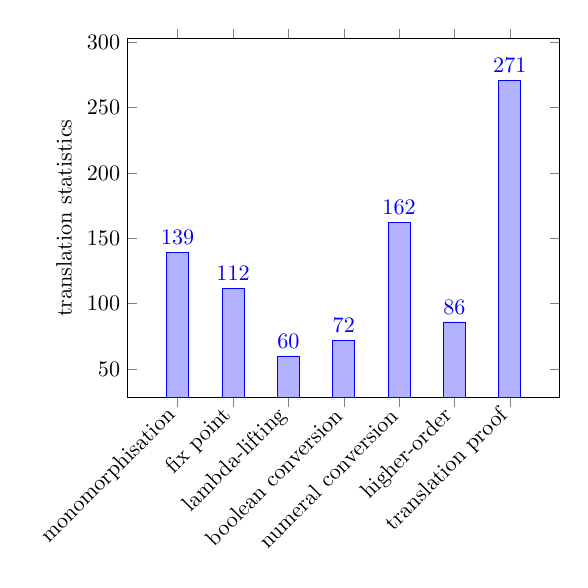
\begin{tikzpicture}[scale=0.8]
\begin{axis}[ybar,enlargelimits=0.15,legend style={at={(2,2)},anchor=north,legend columns=0},ylabel={translation statistics},symbolic x coords={monomorphisation,fix point,lambda-lifting,boolean conversion,numeral conversion,higher-order,translation proof},xtick=data,
nodes near coords,
nodes near coords align={vertical},
x tick label style={rotate=45,anchor=east},]
\addplot coordinates {(monomorphisation,139) (fix point,112) (lambda-lifting,60) (boolean conversion,72)(numeral conversion,162)(higher-order,86)(translation proof,271)};
\end{axis}
\end{tikzpicture}
\end{center}

\noindent Every conversion ($\lambda$-lifting, boolean conversion, numeral conversion and higher-order conversion) is used more than 1 time out of 5, so the code has been tested with a good variety of problems. 
\\The second column shows that 80 percent of the monomorphisation steps reaches a fix point.
\\The last column shows that the translation inside HOL4 was proven 100 percent of the time.
\vspace{5mm}

\noindent To test BEAGLE$\_$TAC's ability to deal with arithmetic without user-provided theorems, we searched through all the problems and removed used-provided arithmetic theorems and see if BEAGLE$\_$TAC could prove them whereas METIS$\_$TAC cannot.
\\There were 65 problems involving arithmetic. All the 79 user-provided arithmetic theorems were removed. This is how BEAGLE$\_$TAC performs on these arithmetic problems.

\begin{center}
\begin{tikzpicture}[scale=2.5]
\newcounter{a}
\newcounter{b}
\foreach \p/\t in {88/unsatifiable, 9/unknown,
                   3/time out}
  {
    \setcounter{a}{\value{b}}
    \addtocounter{b}{\p}
    \slice{\thea/100*360}
          {\theb/100*360}
          {\p\%}{\t}
  }
\end{tikzpicture}
\end{center}

These are the characteristics of these arithmetic problems.
\begin{center}
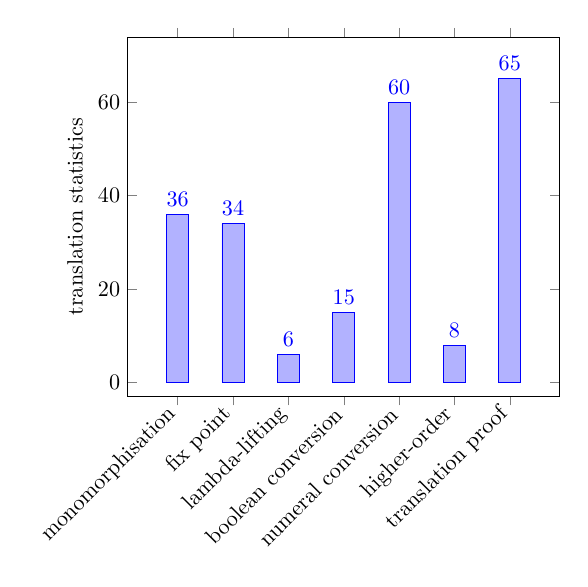
\begin{tikzpicture}[scale=0.8]
\begin{axis}[ybar,enlargelimits=0.15,legend style={at={(2,2)},anchor=north,legend columns=0},ylabel={translation statistics},symbolic x coords={monomorphisation,fix point,lambda-lifting,boolean conversion,numeral conversion,higher-order,translation proof},xtick=data,
nodes near coords,
nodes near coords align={vertical},
x tick label style={rotate=45,anchor=east},]
\addplot coordinates {(monomorphisation,36) (fix point,34) (lambda-lifting,6) (boolean conversion,15)(numeral conversion,60)(higher-order,8)(translation proof,65)};
\end{axis}
\end{tikzpicture}
\end{center}

\section{Contribution and related works}

\subsection{Contribution}
BEAGLE$\_$TAC will be added to the HOL4 library as a TFF converter and and a oracle. It will enables HOL4 user to omit giving arithmetic theorems to "prove" arithmetic goals.

\subsection{Related works}
Here are four different researchers who implemented higher-order to first-order translations:
\begin{enumerate}
\item [-] Joe Hurd developed a translation ~\cite{Hurd03} in his internal prover METIS$\_$TAC. It encodes type variables as first-order logic variables and uses combinators to remove $\lambda$-abstractions. 
\item [-]  Paulson and Meng implemented three different higher-order to first-order translations ~\cite{MengP08} from HOL/Isabelle to the logic of first-order prover.  One of those involves forgetting about the typing information. It leads to an increase of efficiency and a lost of soundness. A "a posterirori" check of the proof is necessary.
\item [-]  Sascha B\"ohme wrote a translation ~\cite{Bohme12} from HOL/Isabelle’s higher-order logic to the first-order logic of SMT solvers which is a monomorphic typed first-order logic.  It performs a monomorphisation step by finding a fix point in a set of special terms. It uses $\lambda$-lifting. It is the translation that has the most similarity with the one we explained in this report.
\item [-] Kaliszyk and Urban developed an automatic tool ~\cite{KaliszykU12} based on HOL light and the Flyspeck project. It includes implementations of sound translations of the HOL Light logic to ATP formalisms: untyped first-order, polymorphic typed first-order, and typed higher-order.
\end{enumerate} 

\noindent Comparatively, our translation outputs monomorphic typed first-order logic formulas in a clause set form. It performs monomorphisation by finding a fix point in a set of constants. It uses lambda-lifting and its higher-order conversion is tweaked to deal with arithmetics. Boolean arguments are instantiated. Non linear-arithmetic terms are treated in a special way as in ~\cite{Bohme12}.

\begin{remark}
To see many different ways of dealing with polymorphic types, you can read \cite{BlanchetteBPS13}.
\end{remark}

\noindent Here are two projects which make use of higher-order to first-order conversion and  give ideas how to enhance HOL4 further more:
\begin{enumerate}
\item [-] Chantal Keller developed a cooperation between the interactive theorem prover Coq and SAT/SMT solvers \cite{Keller13}.
\item [-] Jasmin Blanchette developed a tool to generate counterexamples \cite{Blanchette12}. 

\end{enumerate}

\section{Future works}
We present here what could be done to complete and improve the HOL4-Beagle interaction.
\begin{enumerate}
\item Improving the translation in HOL4:
\\- A first improvement will be to generate theorems from HOL4 theories. 
   It would be based on some heuristic which would involve the number of common constants between the problem and the generated theorem \cite{Paulson10}.
\\- A second improvement will be to translate integers, rationals and reals since Beagle supports them.
\\- A third improvement will be to do a less complete but more efficient higher-order conversion by not converting functions that always appear with the same arity.
 
\item Improving the proof output of Beagle:
\\A complete step by step TFF derivation (direct acyclic graph) would be a nice output. But another idea would be to print only relevant steps which would lead to a smaller proof and counter intuitively an easier proof reconstruction as discussed in the next section. 
 
\item Creation of a HOL4 proof replayer:
\\- Once Beagle creates a reasonable proof output, a HOL4 parser may be created to get a HOL4 representation of the proof.
\\- Then, the first idea is to simulate each steps of the proof by a rule. For example, the Split rule may be simulated by the case disjunction rule.
\\Another idea would be to create an all purpose HOL4 rule such as metis in SledgeHammer for HOL/Isabelle \cite{Paulson10}. Only important lemmas will be used to guide the reconstruction of the proof. Although it would be slower than a direct reconstruction, the flexibility gain could outweigh the cost.
\end{enumerate}

\section{Acknowledgements}
During the 3 months and half I spent at NICTA, everyone I met gave me a very warm welcome. My supervisor, Michael Norrish, always led me to a good approach to the problem. Peter Baumgartner and his student Josh Bax spent time explaining me how Beagle works and reviewing some of my errors. I am really thankful to them. Chantal Keller, my supervisor in France, put my problem into perspective and guided me to write my report. It helped me a lot.

\pagebreak

\bibliography{mybib}{}
\bibliographystyle{plain}

\end{document}